\documentclass[a4paper,11pt]{article}

\usepackage[utf8]{inputenc}
\usepackage[top=2cm, left = 2cm , right=2cm , bottom=2cm]{geometry}
\usepackage{amsmath}
\usepackage{graphicx}
\usepackage{float}
\usepackage{listings}
\usepackage[brazil]{babel}

\pagestyle{plain}

\graphicspath{{./Imagens/}}

\begin{document}

\begin{center}
\textbf{Experiência 3} \\
\hspace{5pt}
Prof. Marconi Kolm Madrid \\
EA722 - 2017/2
\end{center}

\begin{center}
Danilo Pereira Titato - RA 122541 \\
Giovani Granzotto Oliani - RA 146253 \\
Pedro Gabriel Calixto Mendonça - RA 118363 \\
\end{center}

\textbf{Exercício 1}

\begin{gather*}
    Y\left(s\right) = \frac{c_0}{s \left(s + c_1\right)} \cdot
        \left(k_p + k_d s\right) \cdot
        \left(R\left(s\right) - Y\left(s\right)\right) \\
    Y\left(s\right) \cdot \left[1 +
        \frac{c_0 \left(k_p + k_d s\right)}{s \left(s + c_1\right)} \right] =
        R\left(s\right) \cdot \left[
        \frac{c_0 \left(k_p + k_d s\right)}{s \left(s + c_1\right)} \right] \\
    Y\left(s\right) \cdot \left[\frac{s^2 + \left(c_1 + k_d c_0\right)s +
        k_p c_0}
        {s \left(s + c_1\right)}\right] =
        R\left(s\right) \cdot \left[
        \frac{c_0 \left(k_p + k_d s\right)}{s \left(s + c_1\right)} \right] \\
    \frac{Y\left(s\right)}{R\left(s\right)} =
        \frac{k_d c_0 s + k_p c_0}{s^2 + \left(c_1 + k_d c_0\right)s + k_p c_0}
\end{gather*}

\textbf{Exercício 2}

\begin{gather*}
    y\left(\infty\right) = \lim_{s \to 0} s Y\left(s\right) =
        \lim_{s \to 0} s R\left(s\right)
        \frac{k_d c_0 s + k_p c_0}{s^2 + \left(c_1 + k_d c_0\right)s + k_p c_0}
        = \\
    \lim_{s \to 0} s R\left(s\right) \frac{k_p c_0}{k_p c_0} =
    \lim_{s \to 0} s R\left(s\right) = \lim_{s \to 0} s \cdot \frac{1}{s} = 1
\end{gather*}

\textbf{Exercício 3}

\begin{gather*}
    Y\left(s\right) = G_p\left(s\right) \cdot \left\{k_p \left[R\left(s\right) -
        Y\left(s\right)\right] - k_d s Y\left(s\right)\right\} \\
    Y\left(s\right) \cdot \left[1 + G_p\left(s\right) \cdot
        \left(k_p + k_d s\right)\right] =
        k_p \cdot G_p\left(s\right) \cdot R\left(s\right) \\
    \frac{Y\left(s\right)}{R\left(s\right)} = \frac{k_p \cdot G_p\left(s\right)}
        {1 + \left(k_p + k_d s\right) \cdot G_p\left(s\right)} =
        \frac{k_p \cdot \frac{c_0}{s\left(s + c_1\right)}}
        {1 + \left(k_p + k_d s\right) \cdot \frac{c_0}{s\left(s + c_1\right)}}
        = \\
    = \frac{k_p c_0}{s^2 + c_1 s + \left(k_p + k_d s\right) \cdot c_0} =
        \frac{k_p c_0}{s^2 + \left(c_1 + k_d c_0\right)s + k_p c_0}
\end{gather*}

\textbf{Exercício 4}

Usando a fórmula do exercício 3:

\begin{gather*}
    \frac{X_1\left(s\right)}{R\left(s\right)} = \frac{k_p \cdot
        G_p\left(s\right)}{1 + \left(k_p + k_d s\right) \cdot
        G_p\left(s\right)} =
        \frac{k_p \cdot k_{hw} \cdot \frac{1}{m_1 s^2 + c_1 s}}
        {1 + \left(k_p + k_d s\right) \cdot
        k_{hw} \cdot \frac{1}{m_1 s^2 + c_1 s}} = \\
    = \frac{k_{hw} \cdot k_p}
        {m_1 s^2 + c_1 s + \left(k_p + k_d s\right) \cdot k_{hw}} =
        \frac{k_{hw} \cdot k_p}
        {m_1 s^2 + \left(c_1 + k_{hw} k_d\right)s + k_{hw} k_p} = \\
        \frac{k_{hw} k_p / m_1}
        {s^2 + \left(\left(c_1 + k_{hw} k_d\right)/m_1\right)s +
        k_{hw} k_p / m_1} .
\end{gather*}

\pagebreak

\textbf{Procedimento experimental - parte 1}

\textbf{2.}

\begin{gather*}
    \omega_n := \sqrt{\frac{k_{hw}k_p}{m_1}} ~ \left(\text{rad/s}\right)
\end{gather*}

Para $\omega_n = \sqrt{2}$ Hz:

\begin{gather*}
    \sqrt{2}~\text{Hz} = \sqrt{\frac{k_{hw}k_p}{m_1}}
        ~ \left(\text{rad/s}\right) \\
    \sqrt{2} \cdot 2\pi ~ \left(\text{rad/s}\right) =
        \sqrt{\frac{k_{hw}k_p}{m_1}} ~ \left(\text{rad/s}\right) \\
    \frac{k_{hw}k_p}{m_1} = 2 \cdot \left(2\pi^2\right) \\
    k_p = 2 \cdot \left(2\pi^2\right) \cdot \frac{m_1}{k_{hw}} \\
    k_p = 0.0149
\end{gather*}

\textbf{6.}
Foi montado um sistema com valores necessários para obter um comportamento de um
oscilador de frequência $\sqrt{2}$ Hz. O gráfico obtido do seu
\textbf{Commanded Position} foi:

\begin{figure}[H]
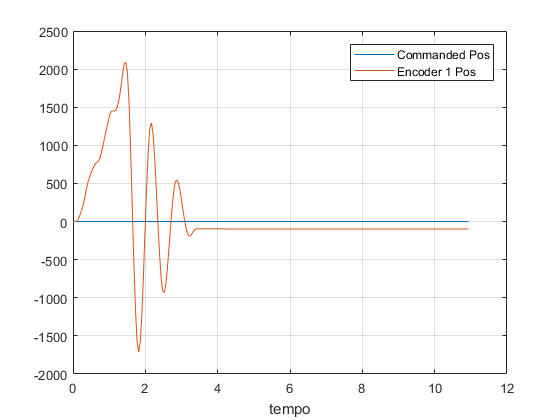
\includegraphics{q04}
\centering
\end{figure}

Usando dois vales da curva, nos instantes de tempo de $1.1815$ e $2.523$,
com diferença de 1 vez o período, temos que a frequência foi de:

\begin{gather*}
    \frac{1}{2.523 - 1.1815} \approx 1.4124~\text{Hz}
        \approx \sqrt{2}~\text{Hz}
\end{gather*}

O sistema teve, então, uma frequência de oscilação excelentemente próxima à
esperada.

Para um ganho proporcional duas vezes maior:

\begin{gather*}
    \omega_n := \sqrt{\frac{k_{hw}k_p}{m_1}} \\
    \omega_n^\prime := \sqrt{\frac{k_{hw}k_p^\prime}{m_1}}, k_p^\prime = 2k_p
        \implies \\
    \omega_n^\prime = \sqrt{\frac{k_{hw} \cdot 2k_p}{m_1}} =
        \sqrt{2} \cdot \sqrt{\frac{k_{hw} k_p}{m_1}} =
        \sqrt{2} \cdot \omega_n
\end{gather*}

Quando o ganho proporcional é dobrado, a sua frequência, então, aumenta num
fator de $\sqrt{2}$. Para um sistema originalmente com $\sqrt{2}$ Hz, sua nova
frequência deverá ser de $\sqrt{2} \cdot \sqrt{2} = 2$ Hz.

Foi montado novamente o sistema, agora com $k_p$ dobrado. A sua resposta foi:

\begin{figure}[H]
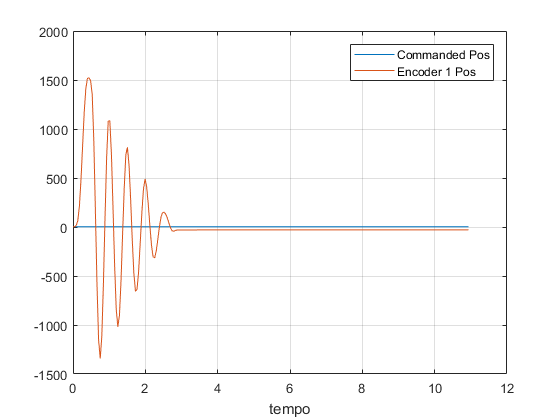
\includegraphics{q06}
\centering
\end{figure}

Usando dois vales da curva, nos instantes de tempo de $0.753$ e $2.258$,
com diferença de 3 vezes o período, temos que a frequência foi de:

\begin{gather*}
    \frac{1}{\left(2.258 - 0.753\right)/3} \approx 1.9934~\text{Hz}
        \approx 2~\text{Hz}
\end{gather*}

O sistema teve, então, uma frequência de oscilação suficientemente próxima à
esperada.

Para se obter um oscilador harmônico perfeito, deve-se ter o fator de
amortecimento $\xi = 0$. Idealmente é capaz de se tê-lo. Porém, em aplicações
reais, é difícil obter-se o valor 0 para $\xi$. Pode-se sempre chegar muito
próximo a zero, mas ainda assim, o sistema não oscila perfeitamente, ele
estabiliza no regime ou explode.

\pagebreak

\textbf{7.}

\begin{gather*}
    \xi := \frac{c_1 + k_{hw} k_d}{2 \sqrt{m_1 k_p k_{hw}}} \\ \\
    \xi = 0 \implies c_1 + k_{hw} k_d = 0 \implies k_d = \frac{-c_1}{k_{hw}} \\
    k_d = -0.00019957 = -1.9957~\text{E-04}
\end{gather*}

A resposta para o sistema com o $k_p$ acima usado foi:

\begin{figure}[H]
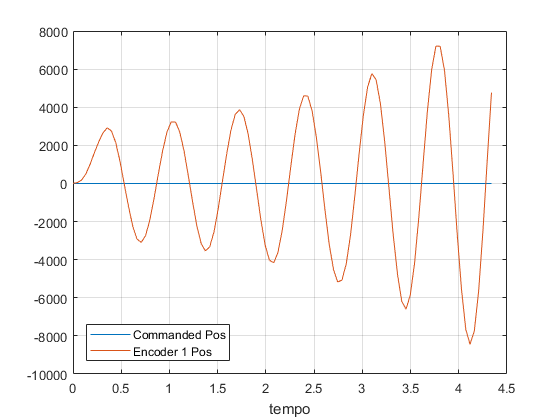
\includegraphics{q07}
\centering
\end{figure}

Como visto, o sistema explodiu. Ele não foi suficientemente controlado e vai ao
infinito. Dificilmente um sistema de controle terá o ganho $k_d$ negativo,
pois ele passa a realimentar positivamente o sistema, proporcionalmente à
velocidade. Logo, sua velocidade aumentará sem fim, como observado no
experimento. \\

\textbf{8.}

\begin{gather*}
    k_d k_{hw} = 50 ~ \text{N.m/s} \implies
        k_d = \frac{50 ~ \text{N.m/s}}{14732 ~ \text{N/m}}
        \approx 0.0034 ~ \text{N.m\textsuperscript{2}/s}
\end{gather*}

\textbf{9.}
Dado que o $k_p$ é zero, não existe mais amortecimento relacionado à posição do
bloco. Desse modo, o bloco não tenta mais retornar à posição inicial.

Porém, apesar de não tentar retornar ao início, nota-se um aumento do
amortecimento, sendo esse um amortecimento viscoso. Ele se dá devido ao aumento
do $k_d$. O $k_d$ está diretamente relacionado ao amortecimento proporcional à
velocidade do bloco. Desse modo, para um mesmo impulso feito pelos participantes
do experimento, o bloco para muito mais rapidamente, devido a um maior
amortecimento para a mesma velocidade de quando num $k_d$ menor, atingindo
velocidades menores ainda e parando antes.

Pode-se ver esse evento na resposta do sistema, onde foram dados empurrões pelos
participantes do experimento:

\begin{figure}[H]
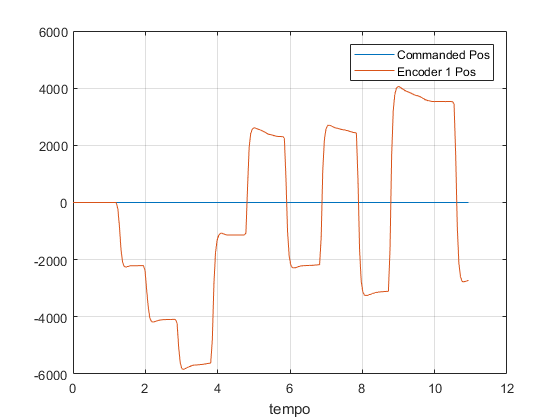
\includegraphics{q09}
\centering
\end{figure}

\textbf{10.}
O novo valor usado para $k_d$ foi de $0.0170$. Como esperado, pela explicação do
item anterior, foi notado um amortecimento maior ainda. Pode-se ver esse evento
na resposta do sistema:

\begin{figure}[H]
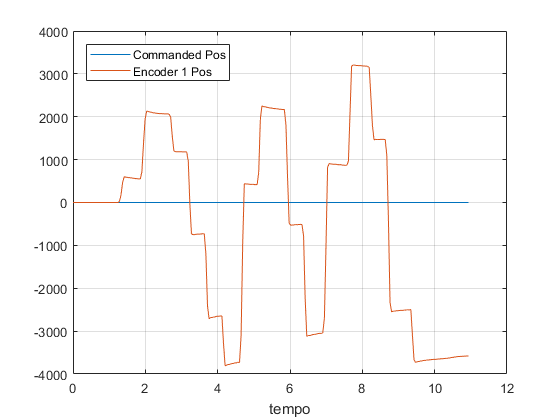
\includegraphics{q10}
\centering
\end{figure}

\pagebreak

\textbf{Procedimento experimental - parte 2}

\textbf{11.}

\begin{gather*}
    \omega_n := \sqrt{\frac{k_{hw} k_p}{m_1}} \implies
        \omega_n^2 = \frac{k_{hw} k_p}{m_1} \implies
\end{gather*}

\begin{equation}
    \label{eq:kp}
    k_p = \frac{m_1}{k_{hw}} \cdot \omega_n^2
\end{equation}

\begin{gather*}
    \xi := \frac{c_1 + k_{hw} k_d}{2 m_1 \omega_n} \implies
        2 \xi m_1 \omega_n = c_1 + k_{hw} k_d \implies
\end{gather*}

\begin{equation}
    \label{eq:kd}
    k_d = \frac{2 m_1 \omega_n \xi - c_1}{k_{hw}}
\end{equation}

Usando as fórmula acima, para uma frequência natural de $\omega_n = 8 \pi$
rad/s, temos:

\begin{itemize}
\item $\xi = 0.2$ (subamortecido) $\implies$
    $k_p = 0.1191, k_d = 0.0017$
\item $\xi = 1.0$ (criticamente amortecido) $\implies$
    $k_p = 0.1191, k_d = 0.0093$
\item $\xi = 2.0$ (sobreamortecido) $\implies$
    $k_p = 0.1191, k_d = 0.0188$
\end{itemize}

\textbf{13.}

\begin{figure}[H]
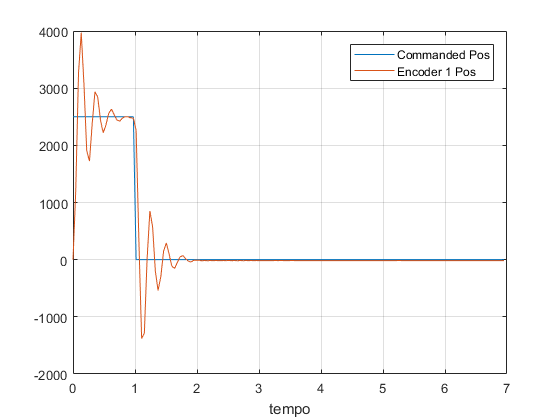
\includegraphics{q13}
\centering
\end{figure}

\pagebreak

\textbf{14.}

\begin{figure}[H]
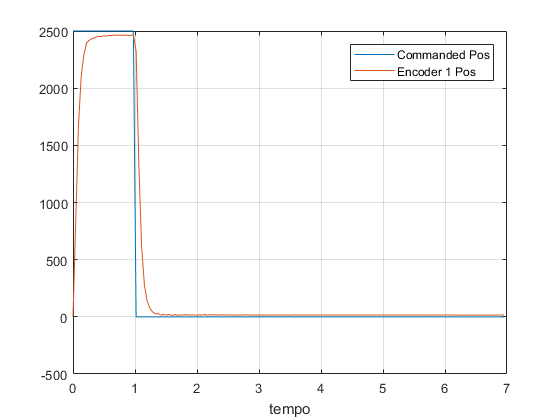
\includegraphics{q14-amort}
\caption{Sistema com controlador criticamente amortecido}
\centering
\end{figure}

\begin{figure}[H]
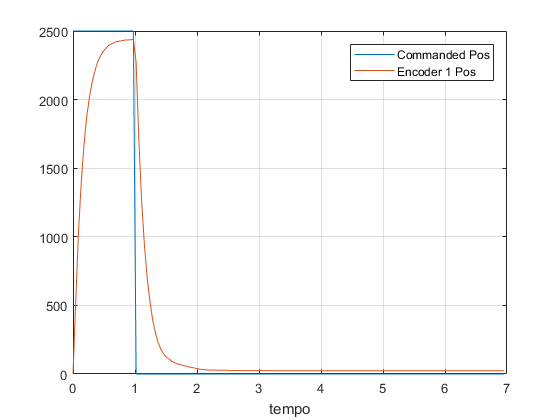
\includegraphics{q14-sobreamort}
\caption{Sistema com controlador sobreamortecido}
\centering
\end{figure}

\textbf{15.}

\begin{gather*}
    M_p := e^{\frac{-\xi \pi}{\sqrt{1 - \xi^2}}} \times 100 ~ \text{(em \%)}
\end{gather*}

Queremos um \textit{overshoot} entre $10\%$ e $20\%$:

\begin{gather*}
    M_p < 20\% \implies e^{\frac{-\xi \pi}{\sqrt{1 - \xi^2}}} < 0.2 \implies
        \frac{-\xi \pi}{\sqrt{1 - \xi^2}} < log\left(0.2\right) \implies
        -\xi \pi < \sqrt{1 - \xi^2} \cdot log\left(0.2\right) \implies \\
        \xi^2 \pi^2 < \left(1 - \xi^2\right) \cdot {log}^2\left(0.2\right)
        \implies \xi^2 \left[\pi^2 + {log}^2\left(0.2\right)\right] <
        {log}^2\left(0.2\right) \implies \\
    \xi < \frac{log\left(0.2\right)}
        {\sqrt{\pi^2 + {log}^2\left(0.2\right)}} \implies
        \xi < -0.4559 \\
    \xi > - \frac{log\left(0.2\right)}
        {\sqrt{\pi^2 + {log}^2\left(0.2\right)}} \implies
        \xi > 0.4559 \\ \\
    M_p > 10\% \implies \\
    \xi > \frac{log\left(0.1\right)}
        {\sqrt{\pi^2 + {log}^2\left(0.1\right)}} \implies
        \xi > -0.5912 \\
    \xi < - \frac{log\left(0.1\right)}
        {\sqrt{\pi^2 + {log}^2\left(0.1\right)}} \implies
        \xi < 0.5912
\end{gather*}

A faixa de $\xi$ é $-0.5912 < \xi < -0.4559$ e $0.4559 < \xi < 0.5912$.
O $\xi$ escolhido foi de $0.5$ (tem que ser positivo para haver amortecimento).
Para calcular o $\omega_n$:

\begin{gather*}
    t_s := \frac{3}{\xi \omega_n} ~ \text{(critério de 5\%)} \\
    \omega_n = \frac{3}{\xi ~ t_s} = \frac{3}{0.5 \cdot 0.5} = 12
\end{gather*}

Usando as equações \ref{eq:kp} e \ref{eq:kd}, obtemos $k_p \approx 0.0272$ e
$k_d \approx 0.0021$. O sistema foi implementado com esses parâmetros e a
resposta obtida foi:

\begin{figure}[H]
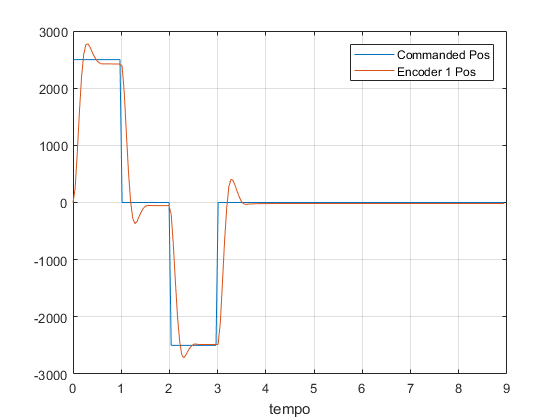
\includegraphics{q15}
\centering
\end{figure}

Para o primeiro pico, o valor de regime foi de $2424$ passos e o pico foi de
$2727$ passos. O \textit{overshoot} foi, então, de
$\frac{2727 - 2424}{2424} = 12.5\%$. Como esperado, o \textit{overshoot} se deu
entre $10\%$ e $20\%$.

Para o instante de tempo de $0.443 s$, temos uma contagem de $2551$ passos, logo
um erro de $\frac{2551 - 2424}{2424} = 5.24\%$.
Para o instante de tempo de $0.487 s$, temos uma contagem de $2490$ passos,
logo um erro de $\frac{2490 - 2424}{2424} = 2.72\%$.
Portanto, o tempo de estabelecimento, para o critério de $5\%$, está entre
$0.443 s$ e $0.487 s$, próximo ao esperado de $0.5 s$.

\end{document}